\documentclass{article}[12pt]
\usepackage{graphicx}
\usepackage{amsmath}
\usepackage{indentfirst}
\usepackage{color}
\usepackage{cite}
\usepackage{wasysym}
\usepackage{amssymb}
\usepackage{multirow}
\usepackage{float}



% --Defining Parameters--
\oddsidemargin -0.25in		% Left margin is 1in + this value
\textwidth 6.75in		% Right margin is not set explicitly
\topmargin -0.25in		% Top margin is 1in + this value
\textheight 9in			% Bottom margin is not set explicitly
\columnsep 0.25in		% separation between columns

% -- Change Section Numbers for Roman Numerals -- 
\renewcommand{\thesection}{\Roman{section}} 
\renewcommand{\thesubsection}{\thesection.\Roman{subsection}}
\renewcommand{\figurename}{Fig.}
\renewcommand\refname{REFERENCES}






\begin{document}

\title{Lab 1}
\author{Samuel Barton}


%--- Heading ---
\begin{center}
\large{\textbf{Lab 1 - The Photoelectric Effect}}\\
\bigskip
\small{\textbf{Partner:} Alexander Knox-Jones; \textbf{Lab Section:} 2 }\\
~\\
Dated: October 2, 2023\\

\end{center}

%--- Abstract ---
\bigskip
\begin{abstract}
  The purpose of this labe was to study the physical phenomenom of the photoelectric effect discovered by Heinrich Hertz which we researched in class.
  Differing from the historical experiment, laser diodes were used to produce monochromatic light to produce a greater intensity of light, and an op-amp to estimate the maximal electron KE without applying an external electic potential.
  In this lab, it was discovered that voltage is independent of light intensity as the value did not change when adjusting the polarizer, and voltage is proportional to frequency. 
  Furthermore, it was discovered that current is proportional to light intensity as well as frequency.
  Using the data collected for different light frequencies, particularly voltage, Planck's constant was estimated to be $ 8.88 \cdot 10^{-34}~\text{J*s} $ which has a percent error of $ 25.3 \% $
\end{abstract}
\bigskip

%--- Introduction ---
\section{Introduction}

In 1887, Heinrich Hertz found that electrons are emitted when electromagnetic radiation shines on a clean, metal surface, hence the photoelectric effect.
He found that the electrons emitted per unit time depends on the frequency and intensity of the light.
This experinent led to Einstein's theory in 1905 that light consists of tiny packets of energy now known as photons, and Planck's Constant was calulated, defining the proportionality constant between energy and EM frequency. 

\begin{equation}
E = h \cdot \nu = KE_{max} + \phi 
\label{main_eq}
\end{equation}

%--- Method ---
\section{Method}

Figure \ref{methods} shows the experimental setup used in this lab to measure the voltage and current of the emitted electrons shows the experimental setup used in this lab to measure the voltage and current of the emitted electrons.
Note that 6 different lasers, each with a distinct wavelength, were used.
The diffuser was used for safety and to spread the light over the cathode. 
The procedure was as follows:

All doors, windows, and any sources of ambient of light were neutralized in order to prevent noise in the data.
An arbitrary laser was mounted on the stand with the plastic diffuser in place.
First, current was measured to identify which light frequencies could produce the photoelectric effect.
First, the current switch was flipped to on, and the voltage switch to off.
Then, with safety goggles in place, one lab partner activated and aimed the laser at the cathode, while the other recorded the current exhibited on the multimeter.
Next, the polarizer was adjusted by a constant rate of 30$ {}^{\circ} $ for a total of 6 current measurements for each laser.
This process was repeated for each laser until currents were measured for each wavelength.
Next, the same process was repeated to measure voltage for each laser.
The polarizer was adjusted for each laser, but it was quicly noticed that this manipulation had no effect on the output voltage, so no extra voltages were recorded.

\begin{figure}[H]
\centering
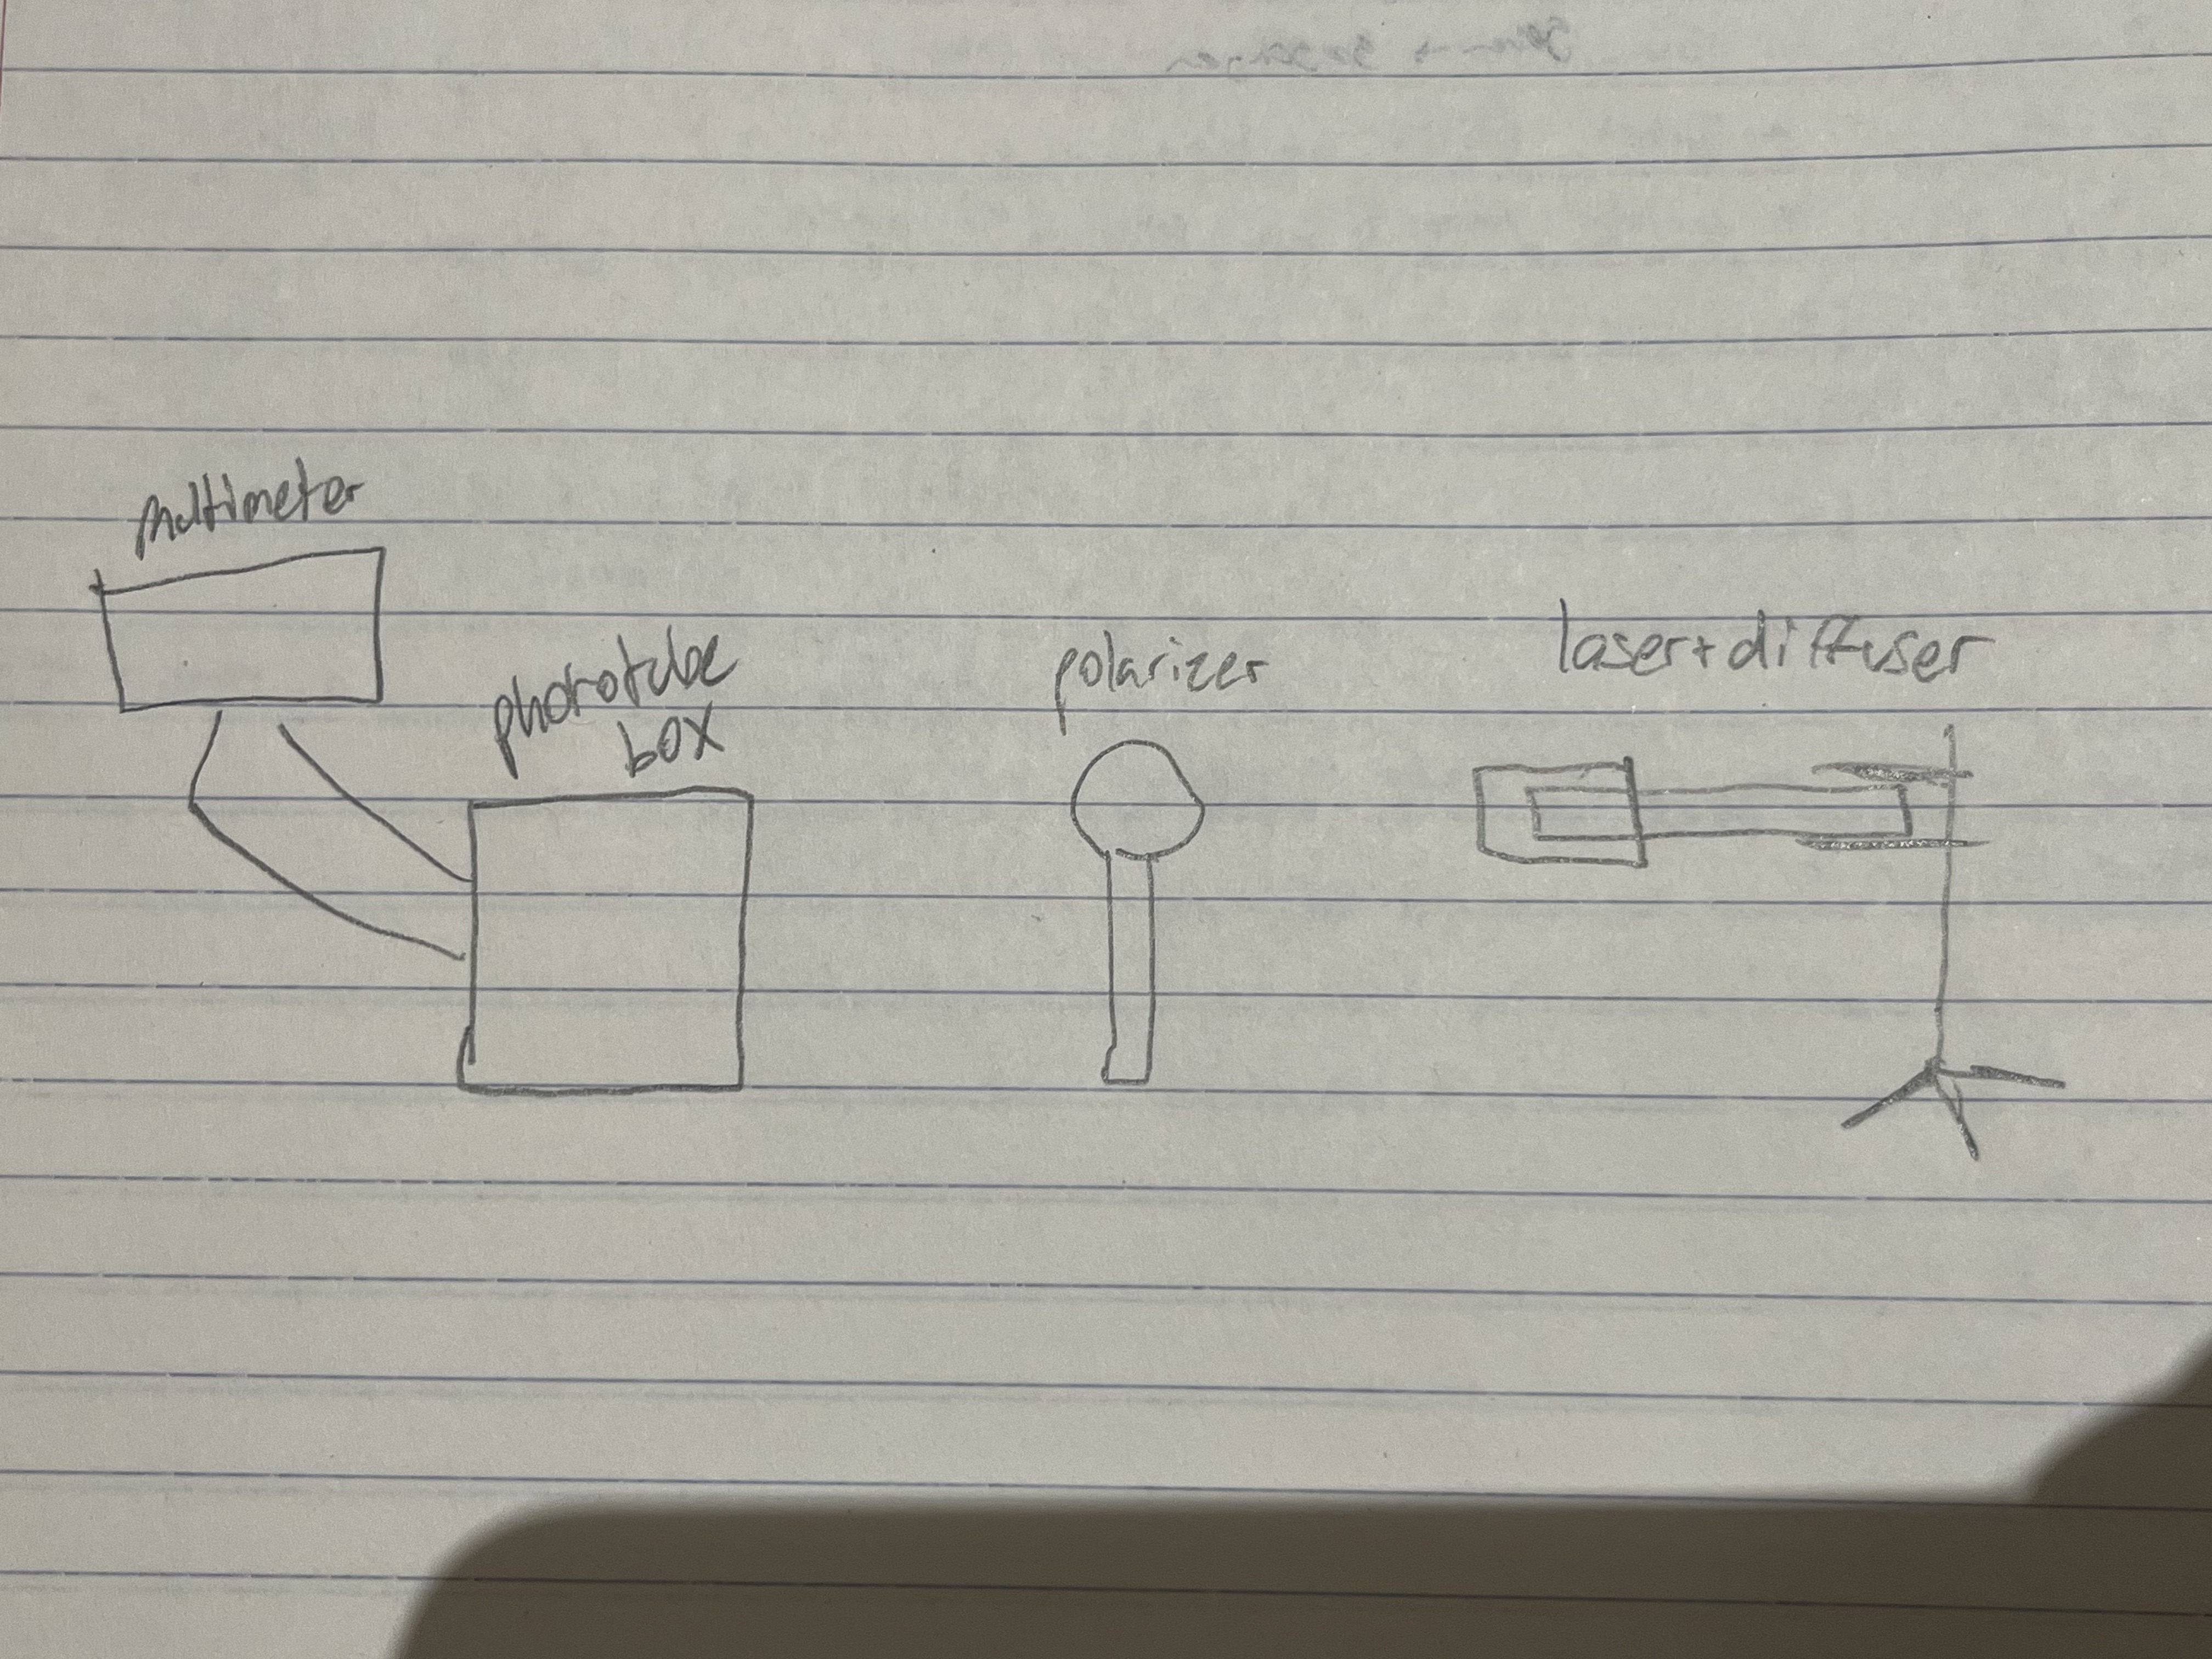
\includegraphics[scale=0.1]{figures/methods.jpeg}
\caption{Diagram of Lab Setup}
\label{methods}
\end{figure}


%--- Data ---
\section{Data}

\begin{table}[H]
\centering
\begin{tabular}{| l | c | c | }

\hline
Polarizer Angle ($ {}^{\circ} $) & Current	& Voltage\\
\hline \hline
90  & 0.143 mA    & 0.202 V \\ \hline
120	&	0.190 mA		&	 \\ 	\hline
150	&	0.125 mA		&	 \\ 	\hline
180 &	0.098 mA		&	 \\	\hline
210 & 0.086 mA    &  \\ \hline
240 & 0.163 mA    &  \\ \hline

\end{tabular}
\caption{Green Laser (532 nm)}
\label{green}
\end{table}

\begin{table}[H]
\centering
\begin{tabular}{| l | c | c | }

\hline
Polarizer Angle ($ {}^{\circ} $) & Current	& Voltage\\
\hline \hline
90  & 0.344 mA    & 0.956 V \\ \hline
120	&	0.254 mA		&	 \\ 	\hline
150	&	0.118 mA		&	 \\ 	\hline
180 &	0.004 mA		&	 \\	\hline
210 & 0.202 mA    &  \\ \hline
240 & 0.392 mA    &  \\ \hline

\end{tabular}
\caption{Blue Laser (445 nm)}
\label{blue}
\end{table}

\begin{table}[H]
\centering
\begin{tabular}{| l | c | c | }

\hline
Polarizer Angle ($ {}^{\circ} $) & Current	& Voltage\\
\hline \hline
90  & 0.232 mA    & 1.151 V \\ \hline
120	&	0.129 mA		&	\\ 	\hline
150	&	0.082 mA		&	\\ 	\hline
180 &	0.007 mA		&	\\	\hline
210 & 0.074 mA    & \\ \hline
240 & 0.156 mA    & \\ \hline

\end{tabular}
\caption{Violet Laser (405 nm)}
\label{violet}
\end{table}

The IR, red, and orange lasers did not produce a current, and thus they were not considered as displaying the photoelectric effect.

\begin{figure}[H]
\centering
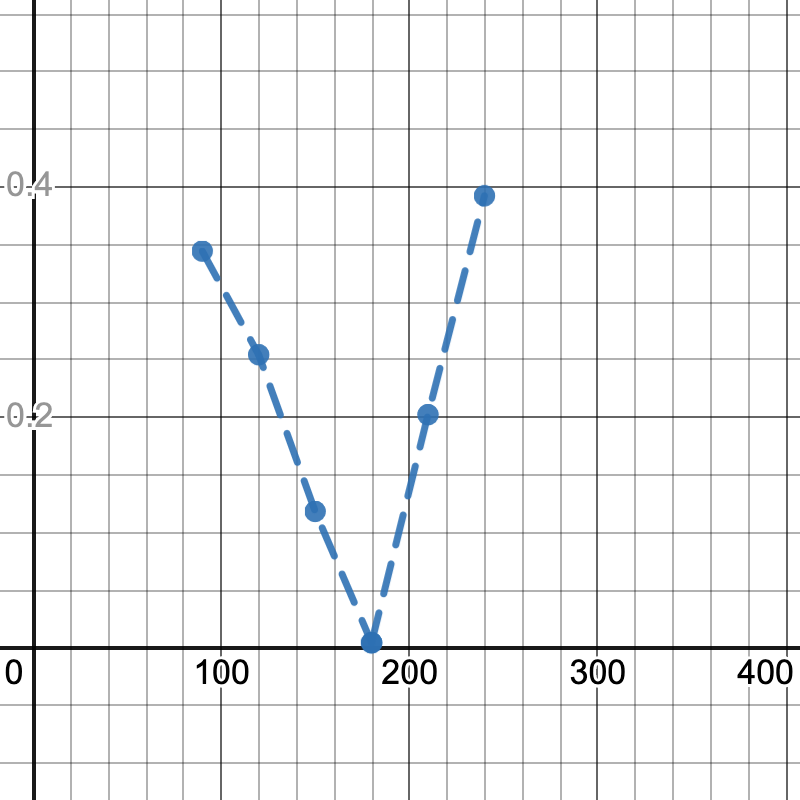
\includegraphics[scale=.4]{figures/currents.png}
\caption{Current vs. Intensity for Blue Light (x-axis: polarizer angle (degrees); y-axis Current (mA))}
\label{currents}
\end{figure}

\begin{figure}[H]
\centering
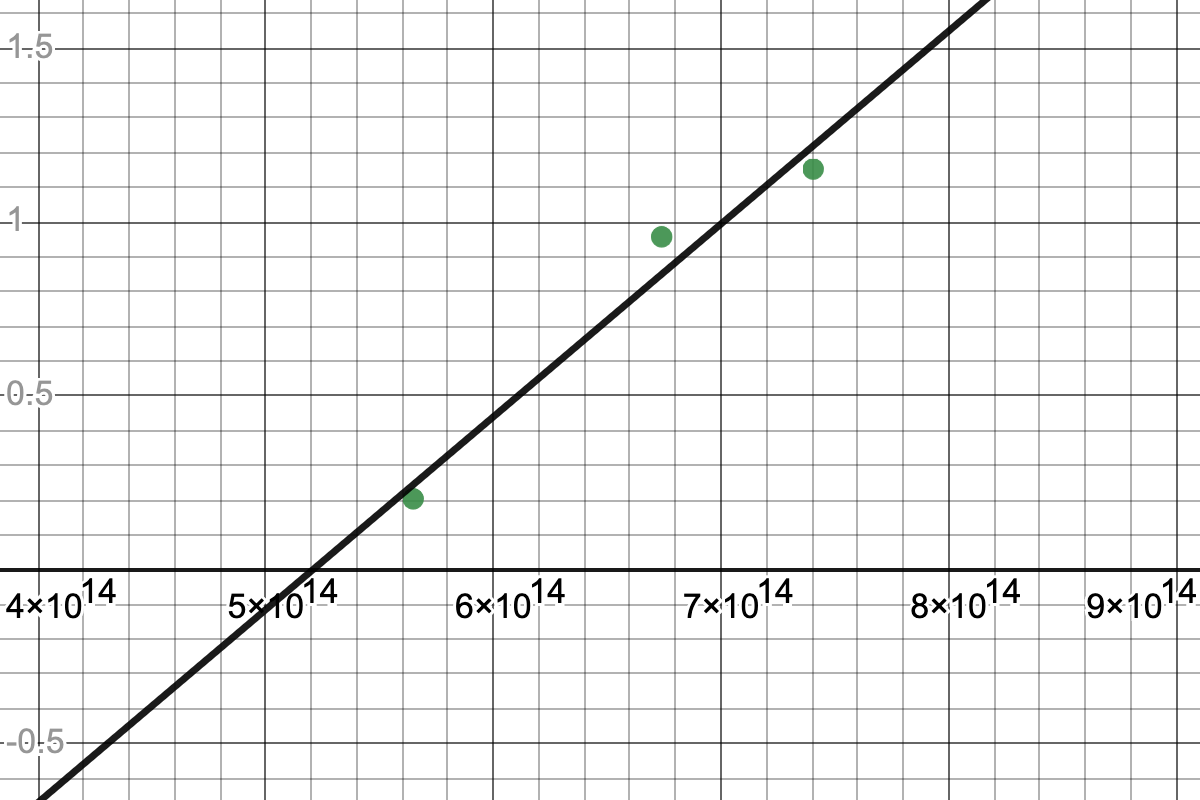
\includegraphics[scale=.4]{figures/plancks.png}
\caption{Calculation of Planck's Constant (x-axis: $ \frac{\text{c}}{\lambda } $ [Hz] y-axis: Energy [V])}
\label{plancks_anal}
\end{figure}

\begin{figure}[H]
\centering
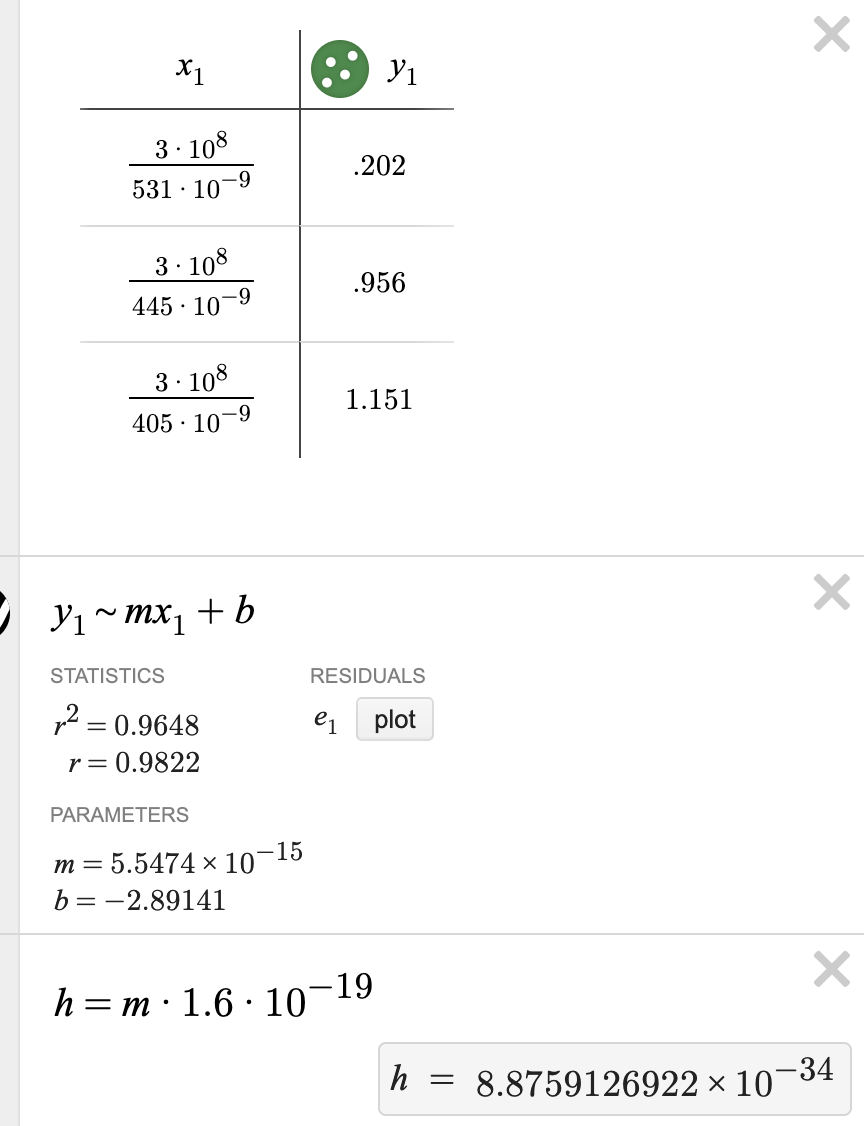
\includegraphics[scale=.4]{figures/planck_calculation.png}
\caption{Calculation of Planck's Constant}
\label{planck_calc}
\end{figure}


\section{Analysis}

Tables \ref{green} - \ref{violet} represent the data collected for all lasers which had a high enough frequency (low-enough wavelength) to exhibit the photoelectic effect (shown by a non-zero current).
Two major questions of the experiment were whether intensity or wavelength have an effect on the energy and number of electrons emitted by the photoelectric effect. 
The data clearly shows that the intensity of the light (manipulated by the polarizer angle) affects the current (number of electrons emitted) but not the voltage (energy).
Additionally, the data shows that the both the current and voltage are dependent on the wavelength, and proportional on frequency (inversely proportional to wavelength).

Figure \ref{currents} displays the relationship between current and intensity.
It can be observed that the current changes somewhat linearly when the intensity is manipulated linearly.
This behavior, though not plotted, is consistent in other data tables.
It can be assumed that, for blue light, the maximum intensity occurs close to 240 degrees since the maximum current occurs at this point. 

With Figure \ref{plancks_anal}, the main goal of this experiment, estimating planck's constant, is achieved.
This plot was produced by calculating frequency with the equation:
\begin{equation}
  \nu = \frac{\text{c}}{\lambda }
\end{equation}
Next, the measured energy (V) was plotted over the frequency, and a linear curvefit was used (see Figure \ref{planck_calc}).
The slope of the curve, $ m $, is in units [V$\cdot$s]
Since we are looking at the maximum KE of an electron, we know the charge to be $ 1.6 \cdot 10^{-19}~\text{C} $ so then Joules can be calculated by multiplying charge and voltage as seen in Figure \ref{planck_calc}.
Henve the value $ h = 8.88 \cdot 10^{-34} $ J*s
From \eqref{main_eq} we have $ E = h \cdot \nu  $, hence $ h $ has units of [J*s], consistent with the calculated value.


%--- Results ---
\section{Results}

The first data tables indicate that intensity does not change the voltage as the measured voltage was a constant when manipulating the polarizer.
Table \ref{blue} and Figure \ref{currents} indicate that current is affected by intensity, however.
Given that there is no constant slope in the rate of change of current over angle, it is assumed that intensity was neither strictly increasing or decreasing, and there was an inflection point around 180 degrees.
Finally, the positive x-intercept Figure \ref{plancks_anal} and the fact that no voltage was calculated for low frequency lasers suggests that there is a minimum frequency threshold to hit before the photoelectric effect is exhibited.
The frequency of the orange light is:
\begin{equation}
  \frac{c}{589*10^{-9}~\text{m}} = 5.093*10^{14}
\end{equation}
A frequency which is less than the x-intercept of $ 5.21*10^14 $, so it makes sense that there was zero current generated by the orange laser.
For the red and IR lasers, with frequencies lower than the orange laser, it is no surprise that there was no current or voltage.

Finally, the value calculated for planck's constant was within the same magnitude of the actual value and has a percent error of $ + 25.3\% $.
This discrepancy between the actual value is likely due to imperfections in in the measurment devices and possibly due to errors/overuse of the cathodes. 

%--- Conclusion ---
\section{Conclusion}

This experiment accomplished the goal of calculating planck's constant using a method similar to Hertz's back in 1887.
Furthermore, this experiment helped gain intuition over the effects of light intensity and wavelength on current and voltage.
There could be improvements going forwards for increasing the accuracy of planck's constant.
More laser wavelengths above the minimum frequency cut-off could have been tested, and lasers with frequencies higher than violet could have been used to create more datapoints. 

\section{References}
\begin{itemize}
  \item Lab Handout
\end{itemize}

%--- Aknowledgements ---
\section{Acknowledgements}

Thanks to TA Bradley for help working out the kinks during the lab procedure!

\end{document}
